In this chapter, the process of geometry generation for the optimization workflow is described. The generated geometry serves as the foundation for simulation using the lattice Boltzmann method described in Chapter \ref{lbm} and is directly defined by the optimization parameters that arise from the used optimization algorithm. 

These parameters are used to dynamically populate predefined geometry templates implemented in Gmsh, a~mesh generation software supporting parametric definition of geometries (associated with the file extension \texttt{.geo}) \cite{gmsh}. The filled template is used to generate an~\texttt{.stl} file. This generated \texttt{.stl} is then loaded into the Trimesh \cite{trimesh} Python package, which voxelizes the geometry based on the specified resolution for the LBM simulation. The voxelized geometry is stored as a 3D NumPy array \cite{numpy}, with options for exporting it in either plain \texttt{.txt} format or the~\texttt{.tnl} format compatible with the TNL library. The~\texttt{.tnl} format offers performance advantages when used with TNL-based LBM implementations.

An overview of the entire process illustrating key steps from parameter definition to simulation-ready output files is presented in Figure \ref{fig:meshgen overview}.


\begin{figure}[H]
	\centering
	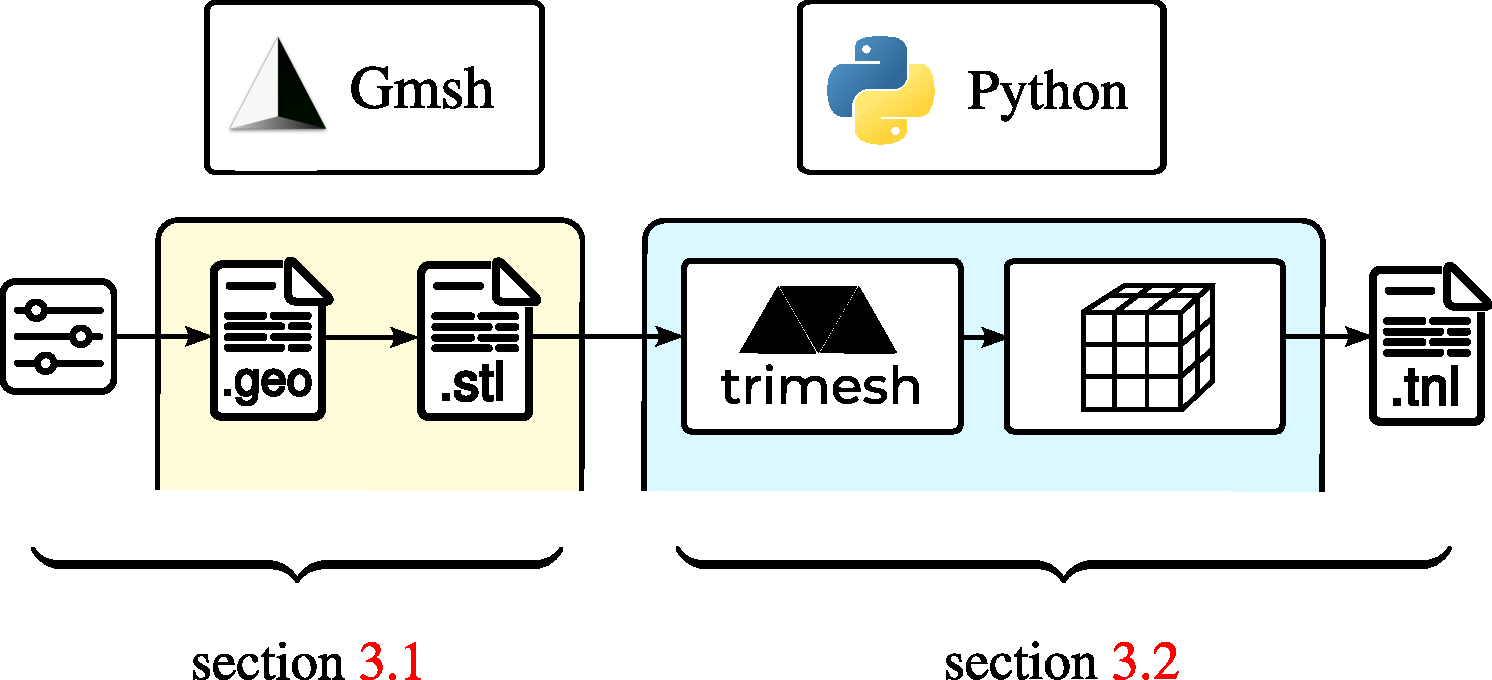
\includegraphics[width=.92\textwidth]{figures/meshgen.pdf}
	\caption{Overview of the geometry generation process. The optimization parameters are used to fill in a Gmsh \text{.geo} template file, which is used to generate an \texttt{.stl} geometry. This geometry is subsequently loaded by the Trimesh Python package and is voxelized and exported either as a \texttt{.tnl} object or a plain \texttt{.txt} file.}
	\label{fig:meshgen overview}
\end{figure}

A custom installable Python package, named \texttt{meshgen}, was implemented to encapsulate the entire process of geometry generation, from defining the geometry templates to preparing the output files for simulations. Its structure reflects the key steps in this process. The Python modules within the package are designed to handle specific tasks, such as loading and processing templates, voxelizing geometries, and providing utility functions. The modules and its specific roles in the process are discussed in detail in the following sections.

Figure  \ref{fig:meshgen structure} provides an overview of the package's structure.  The package is available upon request on Github at \href{https://github.com/buresjan/meshgen}{\texttt{https://github.com/buresjan/meshgen}}.

\begin{figure}[H]
	\centering
	\vspace{6mm}
	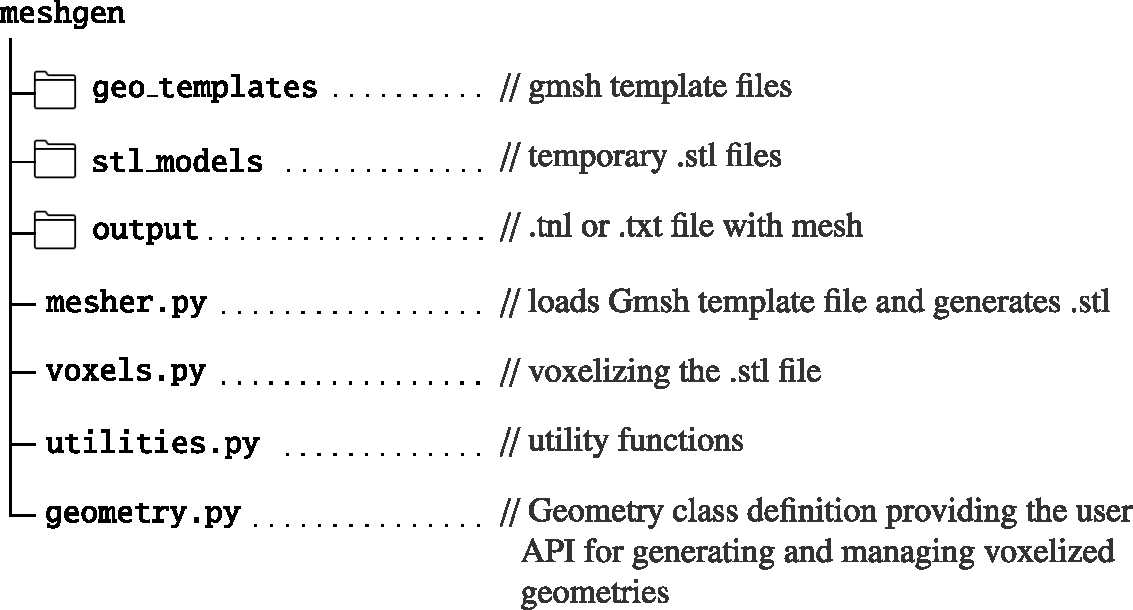
\includegraphics[width=.85\textwidth]{figures/package_overview.pdf}
	\vspace{7mm}
	\caption{Overview of the \texttt{meshgen} package structure. Each module has its specific role in the geometry generation process.}
	\label{fig:meshgen structure}
\end{figure}